\documentclass[tikz,border=6pt]{standalone}
\usepackage{xcolor}
\usepackage{tikz}
\usetikzlibrary{arrows.meta,positioning,calc,fit,backgrounds,shapes.geometric}

\definecolor{panelblue}{HTML}{EAF2FB}
\definecolor{panelred}{HTML}{FCECEC}
\definecolor{panelgray}{HTML}{F4F6F8}
\definecolor{panelgreen}{HTML}{EAF7EF}
\definecolor{accentblue}{HTML}{377EB8}
\definecolor{accentred}{HTML}{D55E5E}
\definecolor{accentgreen}{HTML}{4DAA70}
\definecolor{textgray}{HTML}{555555}
\definecolor{linegray}{HTML}{6F7A86}

\usepackage{lmodern}
\SetSymbolFont{letters}{bold}{OML}{cmbr}{bx}{it}
\renewcommand{\familydefault}{\sfdefault}
\usepackage{sansmathfonts}

\begin{document}
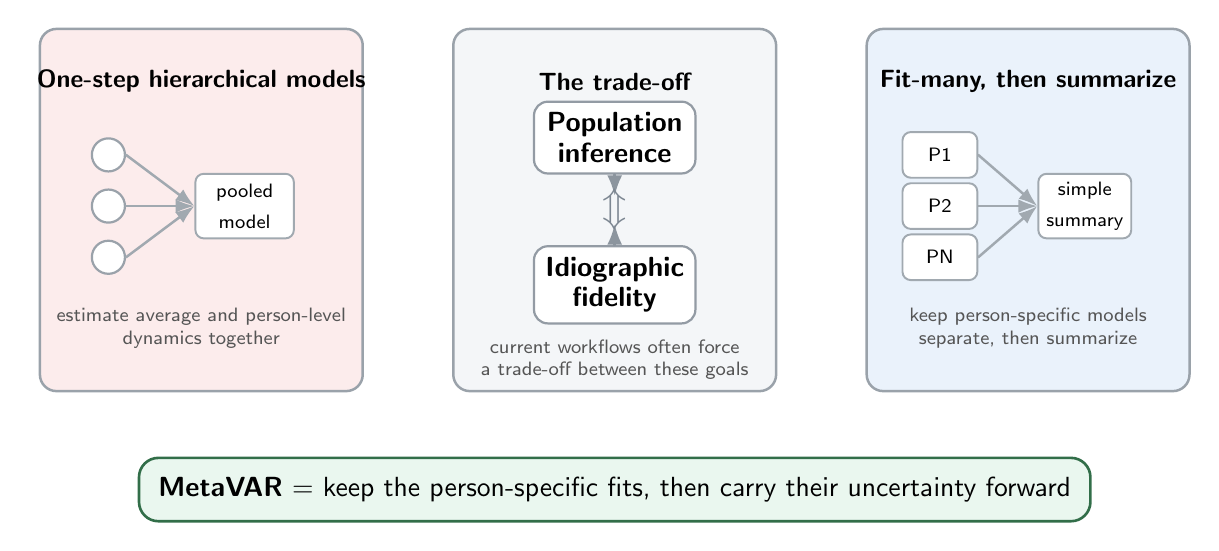
\begin{tikzpicture}[
		x=1cm,y=1cm,
		>=Latex,
		line cap=round,
		line join=round,
		panel/.style={draw=linegray!70, rounded corners=6pt, line width=0.9pt, minimum width=4.1cm, minimum height=4.6cm, inner sep=7pt, align=center},
		smallbox/.style={draw=linegray!65, rounded corners=3pt, line width=0.7pt, fill=white, inner sep=2.5pt, minimum width=0.95cm, minimum height=0.58cm, align=center},
		person/.style={circle, draw=linegray!70, line width=0.8pt, fill=white, minimum size=0.42cm, inner sep=0pt},
		iconlabel/.style={font=\scriptsize, text=textgray, align=center},
		paneltitle/.style={font=\bfseries\small, text=black},
		bodytext/.style={font=\scriptsize, text=textgray, align=left},
		citation/.style={font=\tiny, text=textgray, align=center},
		banner/.style={draw=accentgreen!65!black, fill=panelgreen, rounded corners=7pt, line width=0.95pt, inner sep=7pt, align=center},
		tradebox/.style={draw=linegray!75, fill=white, rounded corners=5pt, line width=0.8pt, inner sep=4pt, align=center},
		flow/.style={-{Latex[length=2.6mm,width=1.9mm]}, line width=0.95pt, draw=linegray!80},
		softflow/.style={-{Latex[length=2.4mm,width=1.7mm]}, line width=0.9pt, draw=linegray!65},
		emphasis/.style={font=\scriptsize\bfseries, text=black}
	]
	
	% Panels
	\node[panel, fill=panelred]   (leftpanel)  at (0,0) {};
	\node[panel, fill=panelgray]  (midpanel)   at (5.25,0) {};
	\node[panel, fill=panelblue]  (rightpanel) at (10.5,0) {};
	\node[banner, minimum width=11.7cm] (bottom) at (5.25,-3.55) {\textbf{MetaVAR} = keep the person-specific fits, then carry their uncertainty forward};
	
	% Left panel title
	\node[paneltitle] at ([yshift=1.63cm]leftpanel.center) {One-step hierarchical models};
	
	% Left icon
	\node[person] (lp1) at ([xshift=-1.18cm,yshift=0.70cm]leftpanel.center) {};
	\node[person] (lp2) at ([xshift=-1.18cm,yshift=0.05cm]leftpanel.center) {};
	\node[person] (lp3) at ([xshift=-1.18cm,yshift=-0.60cm]leftpanel.center) {};
	\node[smallbox, minimum width=1.25cm, minimum height=0.82cm] (lmodel) at ([xshift=0.55cm,yshift=0.05cm]leftpanel.center) {\scriptsize pooled\\[-0.1em]\scriptsize model};
		\draw[softflow] (lp1.east) -- (lmodel.west);
		\draw[softflow] (lp2.east) -- (lmodel.west);
		\draw[softflow] (lp3.east) -- (lmodel.west);
		\node[iconlabel] at ([xshift=0cm,yshift=-1.5cm]leftpanel.center) {estimate average and person-level\\dynamics together};
		
		% % Left bullets
		% \node[bodytext, anchor=west] at ([xshift=-1.65cm,yshift=-1.72cm]leftpanel.center) {$\bullet$ borrow strength across people};
		% \node[bodytext, anchor=west] at ([xshift=-1.65cm,yshift=-2.17cm]leftpanel.center) {$\bullet$ support population inference};
		% \node[bodytext, anchor=west] at ([xshift=-1.65cm,yshift=-2.72cm]leftpanel.center) {$\bullet$ \textbf{but shrink} person-specific\\\hspace*{0.75em}dynamics toward the mean};
		% \node[citation] at ([yshift=-1.93cm]leftpanel.center) {e.g., Asparouhov et al., 2018; Li et al., 2022};
		
		% Middle panel title
		\node[paneltitle] at ([yshift=1.63cm]midpanel.center) {The trade-off};
		\node[tradebox, minimum width=2.05cm, minimum height=0.85cm] (toptrade) at ([yshift=0.92cm]midpanel.center) {\textbf{Population}\\[-0.1em]\textbf{inference}};
			\node[tradebox, minimum width=2.05cm, minimum height=0.85cm] (bottrade) at ([yshift=-0.95cm]midpanel.center) {\textbf{Idiographic}\\[-0.1em]\textbf{fidelity}};
				\draw[flow] (toptrade.south) -- ([yshift=0.18cm]midpanel.center);
				\draw[flow] (bottrade.north) -- ([yshift=-0.18cm]midpanel.center);
				\node[font=\Large, text=linegray!90] at (midpanel.center) {$\Updownarrow$};
				\node[iconlabel] at ([yshift=-1.9cm]midpanel.center) {current workflows often force\\a trade-off between these goals};
				
				% Right panel title
				\node[paneltitle] at ([yshift=1.63cm]rightpanel.center) {Fit-many, then summarize};
				
				% Right icon
				\node[smallbox] (rb1) at ([xshift=-1.12cm,yshift=0.70cm]rightpanel.center) {\scriptsize P1};
				\node[smallbox] (rb2) at ([xshift=-1.12cm,yshift=0.05cm]rightpanel.center) {\scriptsize P2};
				\node[smallbox] (rb3) at ([xshift=-1.12cm,yshift=-0.60cm]rightpanel.center) {\scriptsize PN};
				\node[smallbox, minimum width=1.18cm, minimum height=0.82cm] (ravg) at ([xshift=0.72cm,yshift=0.05cm]rightpanel.center) {\scriptsize simple\\[-0.1em]\scriptsize summary};
					\draw[softflow] (rb1.east) -- (ravg.west);
					\draw[softflow] (rb2.east) -- (ravg.west);
					\draw[softflow] (rb3.east) -- (ravg.west);
					\node[iconlabel] at ([xshift=0cm,yshift=-1.5cm]rightpanel.center) {keep person-specific models\\separate, then summarize};
					
					% % Right bullets
					% \node[bodytext, anchor=west] at ([xshift=-1.65cm,yshift=-1.72cm]rightpanel.center) {$\bullet$ modular and scalable};
					% \node[bodytext, anchor=west] at ([xshift=-1.65cm,yshift=-2.17cm]rightpanel.center) {$\bullet$ preserve idiographic fits};
					% \node[bodytext, anchor=west] at ([xshift=-1.65cm,yshift=-2.72cm]rightpanel.center) {$\bullet$ \textbf{but can ignore} how noisy\\\hspace*{0.75em}person-level estimates are};
					% \node[citation] at ([yshift=-1.93cm]rightpanel.center) {e.g., Epskamp et al., 2018; Lee \& Gates, 2024};
					
					\end{tikzpicture}
\end{document}